\section{Processi di Supporto}
	\subsection{Documentazione}
	    
	    \subsubsection{Scopo}
	    Lo scopo della documentazione è fornire riferimenti precisi ed universali su ogni attività e processo inerenti al progetto. Questa sezione norma come stilare tutti i documenti prodotti durante il ciclo di vita del software. I documenti sono reperibili al seguente repository:
	    \url{https://github.com/CodeOfDutyJS/documentazione}
	    
	    \subsubsection{Aspettative}
	    Le aspettative previste dal processo di Documentazione sono:
	    \begin{itemize}
	    	\item Individuare le norme che permettano al gruppo di scrivere documenti in maniera uniforme;
	    	\item Produzione di documenti chiari, leggibili e facilmente consultabili.
	    \end{itemize}
	    
	    \subsubsection{Descrizione}
	    Questa sezione permette di collezionare tutte le norme che garantiscano una stesura uniforme dei documenti ufficiali.
	    
	    \subsubsection{Ciclo di vita del Documento}
	    \begin{itemize}
	        \item \textbf{Creazione} Il documento viene creato da fonti accettabili e conformamente alle norme. In particolare sono fonti accettabili push sul repository e viene usato un template LaTeX fornito nello stesso;
	        \item \textbf{Implementazione della struttura} Sempre secondo le norme, viene creata la struttura del documento, che deve sempre contenere un registro delle modifiche e un indice che tiene traccia delle voci.
	        \item \textbf{Redazione} il documento viene scritto in forma incrementale, con ogni voce creata interamente;
	        \item \textbf{Revisione} L'implementazione e le modifiche del documento deve seguire gli standard documentativi forniti e devono essere approvate da un membro del gruppo in base al loro formato, adeguatezza, contenuto tecnico e stile di presentazione;
	        \item \textbf{Approvazione della versione} Una volta che il documento contiene tutte le voci descritte nella struttura, viene approvato da un membro del gruppo che non deve aver contribuito precedentemente al documento stesso;
	        \item \textbf{Manuntenzione} Una volta che il documento viene aggiornato come da normativa, viene di nuovo sottoposto a \textbf{Revisione} e \textbf{Approvazione}.
	    \end{itemize}
    
    
    	
	    
	    \subsubsection{Template LaTex e automazione}
	    Allo scopo di uniformare lo stile e velocizzare la produzione dei documenti viene fornito un template LaTeX.
	    \myparagraph{Struttura}
	    Un file "main.tex" raccoglie le sezioni del documento. In testa raccoglie in input un file "package.tex" contenente tutti i package necessari alla compilazione ed un file "config.tex" contenente i comandi di configurazione.
	    \myparagraph{Automazione}
	    Vengono usate le Github Actions per automatizzare la compilazione del file LaTeX in modo da creare un artefatto consultabile da tutto il gruppo ad ogni cambiamento dello stesso ed in modo  da assicurarsi circa la compilazione stessa del file LaTeX. Inoltre uno script Python automaticamente appone l'apposito pedice alle voci da inserire nel glossario.
	    
	    \subsubsection{Pagine}
	    Di seguito una descrizione di pagine sempre presenti nei documenti prodotti dal gruppo.
	    \myparagraph{Frontespizio}
	    Il frontespizio di tutti il documenti del gruppo è descritto nel template LaTeX e contiene dall'alto verso il basso, centrati:
	    \begin{itemize}
	        \item il logo del gruppo;
	        \item il nome del gruppo, seguito da un trattino orrizzontale e il titolo del progetto, entrambi in grassetto;
	        \item il nome del documento in grassetto;
	        \item una tabella a due colonne recante le seguenti voci:
	        \begin{enumerate}
	            \item \textbf{Versione}: la versione del documento;
	            \item \textbf{Approvazione}: lo stato di approvazione, seguito dai nomi dei componenti del gruppo incaricati di tale attività;
	            \item \textbf{Redazione}: i nomi dei componenti del gruppo incaricati di redarre il documento
	            \item \textbf{Verifica}: i nomi dei componenti del gruppo incaricati della verifica del documento
	            \item \textbf{Stato}: lo stadio del ciclo di vita nel quale si trova il documento;
	            \item \textbf{Uso}: può essere interno o esterno;
	            \item \textbf{Destinato a}: i destinatari del documento (lasciare vuoto se ad uso interno)
	        \end{enumerate}
	        \item il recapito mail del gruppo.
	    \end{itemize}
	    
	    \myparagraph{Diario delle modifiche}
	    La seconda pagina contiene sempre il diario delle modifiche: una tabella atta ad elencare ed a descrivere sinteticamente le modifiche in ordine cronologico apposte al documento.
	    Il diario delle modifiche contiene le seguenti voci:
	    \begin{enumerate}
	        \item \textbf{Versione}: la versione del documento;
	        \item \textbf{Data}: la data della modifica, della revisione o approvazione;
	        \item \textbf{Nominativo}: chi ha apportato la modifica, revisione o approvazione;
	        \item \textbf{Ruolo}: chi ha apportato la modifica, revisione o approvazione;
	        \item \textbf{Descrizione}: descrizione suntuaria delle attività effettuate.
	    \end{enumerate}
	    
	    \myparagraph{Indice}
	    Il documento contiene poi sempre un indice ordinato e facilmente consultabile contenente le voci all'interno del documento, in modo da informare sulla struttura dello stesso e di dare modo di trovare velocemente le sezioni ricercate.
	    
	    
	    \myparagraph{Introduzione}
	    Tutti i documenti devono iniziare con una breve sezione d'introduzione volta a spiegare lo scopo del documento e ad inserire eventuali riferimenti.
	    
	    
	    \myparagraph{Intestazione del contenuto}
	    Tutte le pagine di contenuto hanno separata da una linea orizzontale un'intestazione contenente:
	    \begin{itemize}
	        \item a sinistra il logo del gruppo, in versione apposita per intestazione;
	        \item a destra il nome del documento.
	    \end{itemize}
	    
	    
	    \myparagraph{Piè di pagina}
	    il piè di pagina contiene, centrato, i numeri di pagina corrente e pagine totali del documento.
	    
	    
	    \myparagraph{Note}
	    In caso di note, queste vanno numerate per pagina ed essere riportate con la loro numerazione a piè di pagina e descritte il più brevemente possibile.
	    
	    
	    
	    \subsubsection{Norme di stile}
	    
	    \myparagraph{Immagini}
	    Le immagini vanno inserite centrate e fornite di apposita didascalia.
	     
	     
	    \myparagraph{Date}
	    Le date vanno inserite usando il formato YYYY-MM-DD (anno per esteso, mese a due cifre e giorno a due cifre) in conformità all' ISO-8601
	    
	    \myparagraph{Nomi di file}
	    Quando ci si riferisce ad un particolare file, e più in generale tutti i file e le cartelle devono avere nomi chiari, descrittivi del contenuto, ma per quanto possibile sintetici.
	    Per quanto riguarda la convenzione da usare per i nomi, si usa lo Snake Case e si devono seguire le seguenti norme:
	    \begin{itemize}
	        \item tutte le parole da cui è composto il nome devono iniziare con la lettera minuscola;
	        \item nel caso siano presenti date queste sono scritte alla fine del nome seguendo le convenzioni date
	    \end{itemize}
	    
	    \myparagraph{Codice}
	    Tutto il codice riportato nei documenti deve essere scritto con font "typewriter monospaced".
	    
	    \myparagraph{Glossario}
	    Ogni termine riportato nel glossario ha una lettera \textbf{G} maiuscola ed in grassetto apposta sotto il nome. Questa viene apposta automaticamente nel LaTeX del documento da uno script Python in base alle voci presenti nel file glossary.txt presente nella repository, che deve essere aggiornato con tutte le voci presenti nel Glossario.
	    
	    \myparagraph{Stile del testo}
	    \begin{itemize}
	        \item \textbf{Maiuscolo}: vengono scritti per intero in maiuscolo solo gli acronimi;
	        \item \textbf{Corsivo}: vengono scritti in corsivo il nome del gruppo, del proponente, del progetto e dei documenti;
	        \item \textbf{Grassetto}: vengono scritti in grassetto i termini su cui si vuole far ricadere l'attenzione del lettore.
	    \end{itemize}
	    
	    \myparagraph{Riferimenti a documenti}
	    \begin{itemize}
	        \item nel caso il riferimento al documento sia in un titolo come voce di un elenco non si usa il corsivo ma il grassetto.
	        \item ogni qualvolta si fa riferimento al documento in un testo o ad un suo contenuto il nome viene accompagnato, separato da uno spazio, dalla versione, anch'essa in corsivo
	        \item il nome del documento viene scritto per intero, e ogni parola di cui è composto deve iniziare con la lettera maiuscola
	    \end{itemize}
	    
	    \myparagraph{Elenchi}
	    Ogni voce di un elenco può seguire due convenzioni stilistiche:
	    \begin{itemize}
	        \item nel caso la voce non abbia un titolo comincia con la lettera minuscola;
	        \item \textbf{Titolo}: nel caso la voce abbia un titolo questo viene scritto in grassetto, comincia con la lettera maiuscola ed è seguito dai due punti ed da una descrizione.
	    \end{itemize}
	    a discapito della convenzione seguita ogni voce termina con il punto e virgola \textbf{";"} tranne l'ultima che termina con un punto \textbf{"."}, ogni sottoelenco 
	    segue le medesime regole.
	    
	    \myparagraph{Sigle}
	    Nella stesura dei documenti vengono adottate le seguenti sigle:
	    \begin{itemize}
	        \item \textbf{Glossario}: \textbf{G}
	        \item \textbf{Revisione dei Requisiti}: \textbf{RR}
	        \item \textbf{Revisione di Progettazione}: \textbf{RP}
	        \item \textbf{Revisione di Qualifica}: \textbf{RQ}
	        \item \textbf{Revisione di Accettazione}: \textbf{RA}
	        \item \textbf{Responsabile di progetto}: \textbf{Re}
	        \item \textbf{Amministratore}: \textbf{Am}
	        \item \textbf{Analista}: \textbf{An}
	        \item \textbf{Progettista}: \textbf{Pr}
	        \item \textbf{Programmatore}: \textbf{Pg}
	        \item \textbf{Verificatore}: \textbf{Ve}
	    \end{itemize}
	    
	    \subsubsection{Elementi grafici}
	    Di seguito si trovano le norme per gli elementi grafici. Si distinguono due tipi di elementi grafici:
	    \begin{itemize}
	        \item \textbf{Figure}: sono figure le tabelle, i grafici ed i diagrammi UML;
	        \item \textbf{Immagini}: tutti gli altri elementi grafici. 
	    \end{itemize}
	    
	    \myparagraph{Figure}
	    Ogni figura deve essere contrassegnata da una didascalia descrittiva posta al di sotto di essa, seguita da una numerazione progressiva assegnata per sezione. È esente da questa convenzione il diario delle modifiche.
	    la numerazione delle figure è composta da tre cifre \textbf{X.Y.Z}:
	    \begin{itemize}
	        \item \textbf{X.Y}: riferimento alla sezione;
	        \item \textbf{Z}: riferimento progressivo all'interno della sezione.
	    \end{itemize}
	    
	    \myparagraph{Immagini}
	    Le immagini vanno inserite centrate e corredate di didascalia descrittiva sottostante all'immagine stessa.
	    
	    \subsubsection{Procedimento di stesura delle voci}
	    Il seguente diagramma di attività indica il procedimento di stesura delle voci.\\
	    
	    \begin{figure}[hbt!]
	       \centering 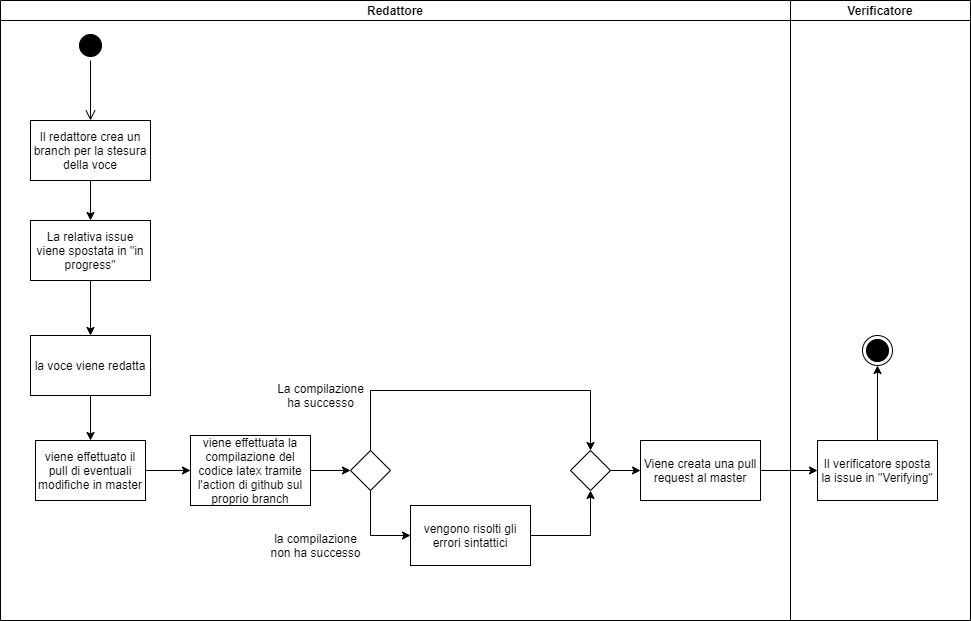
\includegraphics[width=1.0\textwidth]{../_template/images/vociDocumenti.png}
	        \caption{diagramma di attività della stesura delle voci}
	    \end{figure}
	    
	    \subsubsection{Metriche}
		Di seguito vengono elencate le metriche inerenti alla qualità del processo di \textbf{Documentazione}. I valori sono normati nel piano di qualifica. La modalità di rilevazione non è indicata per tutte le metriche: tale dato sarà inserito in fasi successive del progetto.
	    
	    \myparagraph{Gulpease index}
        Rappresenta la leggibilità di un testo valutando la lunghezza delle parole e delle frasi al numero totale di lettere
        \subparagraph{Formula}
        La formula che individua la metrica è:
        \begin{displaymath}
        \textit{IG} = 89 + \frac{300 * \textrm{Frasi} - 10* \textrm{Lettere}}{\textrm{Parole}}
        \end{displaymath}
        Dove:
        \begin{itemize}
        \item[] $IG =$ Gulpease index
        \item[] $\textrm{Frasi} =$ numero complessivo di frasi
        \item[] $\textrm{Lettere} =$ numero complessivo di lettere
        \item[] $\textrm{Parole} =$ numero complessivo di parole
        \end{itemize}
        Per calcolare l'indice viene utilizzato uno script Python, attivato manualmente attraverso una GitHub Action. Il valore viene quindi calcolato utilizzando i documenti presenti in un preciso momento all'interno della repository.
        
        \myparagraph{Correttezza ortografica}
        Rappresenta il numero totale di errori ortografici presenti. Essendo un valore intero che non è composto da altri sottoelemento non ha una formula
        \mysubparagraph{Modalità di rilevazione}
        Viene calcolato durante la verifica di un documento.
	    
	    
	    \subsubsection{Strumenti}
	    \myparagraph{LaTeX}
	    Viene usato LaTeX come linguaggio markdown per rendere più semplice ed uniformare la scrittura collaborativa dei documenti.
	    \myparagraph{TexLive}
	    Per la stesura dei documenti e la loro compilazione.
	    \myparagraph{Overleaf}
	    Per la stesura dei documenti.

	\subsection{Gestione della configurazione}
		
		\subsubsection{Scopo}
		Lo scopo della configurazione è quello di mantere un ordine tra il software prodotto e la relativa documentazione. Ogni elemento che viene configurato dispone di:
			\begin{itemize}
				\item uno stato identificativo che dà informazioni sullo stato dell'elemento
				\item una locazione precisa nel quale può essere reperito
			\end{itemize}
		Inoltre, ogni elemento viene modificato secondo procedure note e sottoposto a versionamento.
		
		\subsubsection{Aspettative}
		\begin{itemize}
			\item permettere una stesura sistematica di codice e documentazione;
			\item classificare i prodotti in maniera uniforme in base allo stato nel quale essi si trovano;
			\item permettere di tracciare i cambiamenti apportati ai prodotti.
		\end{itemize}
		
		\subsubsection{Descrizione}
		Il processo di Gestione della configurazione permette di raggruppare ed organizzare gli strumenti utilizzati per la stesura di documenti e codice. Inoltre definisce gli aspetti riguardanti il versionamento e la coordinazione del gruppo.
		
		\subsubsection{Versionamento}
			
			\myparagraph{Codice di versione del documento}
			Per tenere traccia di ogni documento, il gruppo ha deciso di ricorrere al seguente formato di versione \textbf{X.Y.Z}, dove:
			\begin{itemize}
				
				\item \textbf{X}: indica una versione del documento stabile, dove è stata chiaramente definita e implementata la struttura. Incrementi a questo numero devono essere fatti quando la struttura stessa cambia, sia per aggiunta o rimozione di voci. Indica inoltre una versione validata dal responsabile di progetto ed esposta al pubblico.
				
				\item \textbf{Y}: indica la completa implementazione di una sezione del documento e corrispettiva verifica, o il completamento di una lista pianificata di correzioni.
				
				\item \textbf{Z}: indica un cambiamento minore o correzione verificato/a del documento.
			\end{itemize}
			
			\myparagraph{Codice di versione del codice}
			Per tenere traccia del codice, il gruppo ha deciso di adottare il versionamento semantico, con il seguente formato di versione \textbf{X.Y.Z}, dove:
			\begin{itemize}
			    \item \textbf{X}: indica una versione dove l'API pubblica è considerata stabile; la versione 0 indica una API instabile. La definizione dei contratti d'interfaccia dovrebbe essere conosciuta a priori e definita tramite documentazione o definita dal codice stesso.
			    \item \textbf{Y}: la versione Y deve essere incrementata se viene implementata completamente una funzionalità retrocompatibile, o se una funzionalità dell'API è marcata come deprecata. la versione Z deve essere riportata a 0 quando questa viene incrementata. essa può comprendere miglioramenti a funzionalità già esistenti.
			    \item \textbf{Z}: la versione Z indica modifiche atte a correggere comportamenti errati (bug) del'API.  
			\end{itemize}
			
			ogni incremento al codice di versionamento avviene a posteriori del completamento di un processo di verifica. L'incremento della versione Y comporta, oltre al completamento del processo di verifica il completamento di un processo di validazione.  
			
			\myparagraph{Tecnologie}
			Come sistema di versionamento è stato scelto Git, il quale dispone del servizio Github per ospitare la repository remota. Altro strumento interessante messo a disposizione da Github è "Github Actions" il quale permette di realizzare un servizio di Continuous Integration.
			
			\myparagraph{Repository}
			Per interagire con il sistema di versionamento scelto, ogni componente del gruppo può utilizzare la versione da linea di comando (Git) con opportuni plugin per facilitare l'uso del sistema di versionamento. Alternativamente è possibile utilizzare la versione GUI fornita su Github.\\
			La repository dei documenti è disponibile all'indirizzo:\\
			\begin{center}
				\url{https://github.com/CodeOfDutyJS/documentazione}
			\end{center}
			La repository del codice è disponibile all'indirizzo:\\
			\begin{center}
				\url{https://github.com/CodeOfDutyJS/hdviz}
			\end{center}
			
			\myparagraph{Struttura del repository}
			All'interno del repository è possibile trovare:
			\begin{itemize}
				\item \textbf{nome-del-documento}: tutti i documenti sono disponibili al livello più esterno del repository.
				\item \textbf{\_config e \_template}: permettono la gestione separata della configurazione dei file .tex
				\item \textbf{.gitignore}: elenca tutti i file da escludere dal versionamento.
				\item \textbf{glossario.txt}: elenca tutte le parole all'interno del glossario
				\item \textbf{\_glo\_replace.py}: script in python che genera un pedice G ad ogni occorenza di tutte le parole presentiin "glossario.txt"
			\end{itemize}
			
			\myparagraph{Estensione dei file}
			Per la documentazione saranno utilizzati solamente le seguenti estensioni di file:
			\begin{itemize}
				\item file con estensione .pdf (l'elaborato da consegnare);
				\item file con estensione .tex per la gestione dei documenti in Latex;
				\item immagini e file ausiliari di supporto
			\end{itemize}
		
			\myparagraph{Branching}
			Ogni repository verrà gestito in branch ovvero spazi di lavoro separati che permettono di lavorare sul materiale all'interno del repository mantenendo le modifiche di ogni utente nel suo branch personale. Perciò all'interno di ogni repository saranno presenti:
			\begin{itemize}
				\item \textbf{Branch master}: branch all'interno del quale viene raccolto il lavoro verificato, e quindi disponibile al rilascio
				\item \textbf{Branch personali}: branch utilizzati come aree di lavoro per i membri del gruppo.
			\end{itemize}
			Il lavoro verrà trasferito da un branch personale al branch master solamente quando il lavoro compiuto all'interno del branch personale verrà verificato tramite una Pull Request. Essa permette di tenere il lavoro in uno "spazio separato" per essere verificato, corretto e successivamente fuso con il ramo master in caso di verifica positiva.
			
			\myparagraph{Gestione delle modifiche}
			I membri del gruppo possono modificare i file presenti all'interno di ogni branch personale. È consigliato utilizzare la funzione di commit presente in Git per tenere traccia di ogni cambiamento nella struttura del repository e per identificare l'autore di un determinato cambiamento. Per modificare contenuti e strutture dei file è consigliato contattare il responsabile del file che si vuole modificare, proporre la modifica, e in caso di approvazione effettuare tali modifiche. Nel caso di errori grammaticali è possibile correggere autonomamente i documenti. 
	\subsubsection{Project manager}
        Al fine di gestire le dipendenze ed uniformare ed automatizzare le attività di analisi statica del codice e di esecuzione dei test il gruppo ha deciso di adottare yarn.
	\subsection{Gestione della Qualità}
		\subsubsection{Scopo}
		Lo scopo è quello di assicurare che il prodotto realizzato offra i servizi richiesti dal cliente, e che essi rispettino gli obbiettivi di qualità prefissati.
		
		\subsubsection{Aspettative}
		Gli obbiettivi della gestione della qualità sono i seguenti:
		\begin{itemize}
			\item qualità del prodotto;
			\item qualità all'interno dell'organizzazione e in particolare nei suoi processi;
			\item soddisfazione del cliente e proponente
		\end{itemize}
		
		\subsubsection{Descrizione}
		La trattazione approfondita della gestione della qualità è presente all'interno del \textit{Piano di Qualifica v2.0.0}, all'interno del quale sono descritti tutti i protocolli utilizzati per garantire la qualità durante lo sviluppo del progetto. All'interno di tale documento in particolare sono approfonditi:
		\begin{itemize}
			\item gli standard utilizzati;
			\item i processi di interesse negli standard;
			\item gli attributi del software più significativi per il progetto
		\end{itemize}
		In particolare per ogni processo:
		\begin{itemize}
			\item gli obbiettivi da raggiungere;
			\item le metodologie da applicare;
			\item le metriche da utilizzare
		\end{itemize}
		
		\subsubsection{Attività}
		Le tre attività che caratterizzano il processo sono:
		\begin{itemize}
			\item \textbf{Pianificazione}: prefissare obbiettivi di qualità e definire metodologie per perseguirli. È inoltre necessario impiegare in maniera efficiente le risorse a disposizione (materiali e umane)
			\item \textbf{Valutazione}: applicare ciò che è stato definito nella Pianificazione, monitorando e misurando i risultati
			\item \textbf{Reazione}: in base ai risultati ottenuti, adattare le metodologie
		\end{itemize}
		
		\subsubsection{metriche di qualità del prodotto}
		\myparagraph{Correttezza dello scambio dei dati}
        Il prodotto software ha bisogno di dati provenienti da fonti esterne. Questa 
        metrica misura che i dati ricevuti da tali fonti non siano modificati o errati 
        in qualsiasi modo. Per dato si intende l'informazione più atomica possibile
        \textit{ESEMPIO: in una banca dati anagrafica un dato può essere la data di 
        nascita, oppure il cognome.}
        \subparagraph{Formula}
        La formula che individua la metrica è:
        \begin{displaymath}
          D_{err} = \#\ di\ errori
        \end{displaymath}
        Dove:
        \begin{itemize}
        \item[]$D_{err} =$  numero di errori totali rilevati sui dati importati 
        nell'applicativo.
        \end{itemize}
        \myparagraph{Densità di errori}
        Indica il numero di errori rilevati sul codice tramite i test di unità, è una 
        misura del rapporto tra il totale dei test di unità errati e il totale dei test 
        di unità eseguiti.
        \subparagraph{Formula}
        \begin{displaymath}
          E_{density} = A_{err}/B_{tests}
        \end{displaymath}
        Dove:
        \begin{itemize}
          \item[] $E_{density} =$ densità di errori;
          \item[] $A_{err} =$ totale test di unità errati;  
          \item[] $B_{tests} =$ totale test di unità eseguiti.
        \end{itemize}
        
        \myparagraph{Qualità della messaggistica}
        È una metrica che indica la chiarezza dei messaggi di errore o di avviso 
        all'utente. Per essere chiaro un messaggio deve avere le seguenti 
        caratteristiche:
        \begin{itemize}
          \item deve indicare qual è l'errore, o il motivo dell'avviso;
          \item deve indicare una o più azioni correttive.
        \end{itemize}
        Messaggi che non rispettano le suddette caratteristiche non saranno considerati 
        chiari.
        \subparagraph{Formula}
        \begin{displaymath}
          Q_{mex} = A_{clear}/B_{tot}
        \end{displaymath}
        Dove:
        \begin{itemize}
          \item[] $Q_{mex} =$ qualità della messaggistica;
          \item[] $A_{clear} =$ totale messaggi considerati chiari; 
          \item[] $B_{tot} =$ totale messaggi all'utente.
        \end{itemize}
        \mysubparagraph{Modalità di rilevazione}
        Gli avvisi e gli errori segnalati all'utente sono contati manualmente.
        
        \myparagraph{Numero di click}
        Conta il numero di click necessari per completare uno specifico task. Il task 
        in analisi è il seguente: 
        \begin{itemize}
          \item click necessari per importare un set di dati nell'applicativo.
        \end{itemize}
        \textit{Sarà fornita una descrizione più precisa del task in fasi successive 
        dell'attività di progetto.}
        \subparagraph{Formula}
        \begin{displaymath}
          C_{click}(t) = \#\ di\ click
        \end{displaymath}
        Dove:
        \begin{itemize}
          \item[] $C_{click} =$ indica il numero totale di click per completare il 
        task; 
          \item[] $t =$ è il task da misurare.
        \end{itemize}
        \subparagraph{Modalità di rilevazione}
        Per ottenere valori ai fini della metrica saranno eseguiti dei test 
        sull'applicativo in funzione.
        
        \myparagraph{Site depth}
        È la profondità dell'albero che rappresenta la struttura dell'applicativo.
        \subparagraph{Formula}
        \begin{displaymath}
          S_{depth} = td(G)
        \end{displaymath}
        Dove:
        \begin{itemize}
          \item[] $S_{depth} =$ è la profondità della struttura del prodotto;
          \item[] $td(G) =$ è la funzione che calcola la massima profondità (tree 
        depth).
        \end{itemize}
        
        \myparagraph{Response time}
        Metrica di tempo che misura la durata di uno specifico task in secondi. Il 
        task misurato è:
        \begin{itemize}
          \item caricamento di un set di dati all'interno del progetto.
        \end{itemize}
        \textit{In fasi successive del progetto saranno fornite ulteriori specifiche 
        riguardanti al task (ad esempio quale set di dati viene utilizzato per la 
        misurazione).}
        \subparagraph{Formula}
        \begin{displaymath}
          T_{response} = B_{end}-A_{start}
        \end{displaymath}
        Dove:
        \begin{itemize}
          \item[] $T_{response} =$ durata totale del task;
          \item[] $B_{end} =$ termine del task;
          \item[] $A_{start} =$ inizio del task.
        \end{itemize}
        
        \myparagraph{Complessità ciclomatica}
        La complessità ciclomatica è la misura della quantità dei possibili percorsi di 
        branching di una porzione di codice. Il codice è rappresentato tramite un 
        grafo orientato con un nodo di start e finish dove gli altri nodi rappresentano 
        istruzioni decisionali, la complessità ciclomatica è quindi il numero di 
        cammini lineari indipendenti dal nodo start al nodo finish.
        \subparagraph{Formula}
        \begin{displaymath}
          v(G) = e - n + 2p
        \end{displaymath}
        Dove:
        \begin{itemize}
          \item[] $v(G) =$ complessità ciclomatica del grafo G;
          \item[] $e =$ numero di archi del grafo;
          \item[] $n =$ numero di nodi del grafo;
          \item[] $p =$ numero di componenti connesse.
        \end{itemize}
        
        \myparagraph{Indipendenza dei test}
        Questa metrica misura l'indipendenza dei test, ossia:
        \begin{itemize}
          \item un test non deve fare affidamento su altri test o elementi esterni;
          \item un test deve essere ripetibile e il suo risultato deve rimanere 
        invariato.
        \end{itemize}
        \subparagraph{Formula}
        \begin{displaymath}
          I_{test} = A_{ind}/B_{tests}
        \end{displaymath}
        Dove:
        \begin{itemize}
          \item[] $I_{test} =$ è l'indice di indipendenza dei test;
          \item[] $A_{ind} =$ numero di test considerati indipendenti;
          \item[] $B_{tests}$ numero totale di test.
        \end{itemize}
        
        \myparagraph{Facilità di comprensione}
        È un indice che misura la facilità di comprensione del codice. Un codice 
        sorgente facilmente comprensibile avrà bisogno di meno commenti, viceversa 
        codice complicato avrà più commenti.
        \subparagraph{Formula}
        \begin{displaymath}
          F_{compr} = A_{comm}/SLOC
        \end{displaymath}
        Dove:
        \begin{itemize}
          \item[] $F_{compr} =$ indice della facilità di comprensione;
          \item[] $A_{comm} =$ numero totale di righe di commento;
          \item[] $SLOC =$ numero di righe del codice sorgente.
        \end{itemize}
        
        \myparagraph{Sfin}
        Structural Fan-In, indica il numero di procedure che chiamano una specifica 
        procedura. L'oggetto della misura sono le unità architetturali.
        \subparagraph{Formula}
        \begin{displaymath}
          sfin(u) =  \sum u_{caller}
        \end{displaymath}
        Dove:
        \begin{itemize}
          \item[] $sfin(u) =$ calcolo dello sfin dell'unità $u$;
          \item[] $\sum u_{caller} =$ somma delle unità che utilizzano $u$.
        \end{itemize}
        
        \myparagraph{Sfout}
        Structural Fan-Out, indica il numero di procedure di cui necessita una 
        specifica procedura. L'oggetto della misura sono le unità architetturali. 
        \subparagraph{Formula}
        \begin{displaymath}
          sfout(u) = \sum u_{callee}
        \end{displaymath}
        Dove:
        \begin{itemize}
          \item[] $sfout(u) =$ calcolo dello sfout dell'unità $u$;
          \item[] $\sum u_{callee} =$ somma delle unità utilizzate da $u$.
        \end{itemize}
		
		\subsubsection{Metriche}
		Di seguito vengono elencate le metriche inerenti alla qualità del processo di \textbf{Gestione della qualità}. I valori sono normati nel piano di qualifica. La modalità di rilevazione non è indicata per tutte le metriche: tale dato sarà 
        inserito in fasi successive del progetto.
		\myparagraph{Percentuale di metriche soddisfatte}
        Indica la percentuale in centesimi del numero di metriche con valore soddisfacente. Una basso valore percentuale è indice quindi di una bassa qualità.
        \subparagraph{Formula}
        \begin{displaymath}
          PMS = \frac{\textrm{Soddisfatte}}{\textrm{Totali}}
        \end{displaymath}
        Dove:
        \begin{itemize}
        \item[] $PMS =$ Percentuale di metriche soddisfatte
        \item[] $\textrm{Soddisfatte} =$ numero totale di metriche con valore soddisfacente
        \item[] $\textrm{Totali} =$ numero totale di metriche calcolate
        \end{itemize}
    \subsubsection{Strumenti}
		Gli strumenti utilizzati per la qualità sono:
		\begin{itemize}
			\item \textbf{Standard ISO-12207};
			\item \textbf{Standard ISO-9126};
			\item \textbf{Metriche}
		\end{itemize}
	
	\subsection{Verifica}
	\subsubsection{Scopo}
	Lo scopo del processo di verifica è dare prova materiale che un sistema o un elemento del sistema soddisfa i requisiti e specifiche richiesti.
	
	\subsubsection{Aspettative}
	\begin{itemize}
		\item garantire che i prodotti rispettino i requisiti prefissati e le specifiche richieste;
		\item garantire la qualità dei prodotti ottenuti dai vari processi;
		\item permettere di procedere alla fase di validazione.
	\end{itemize}

	\subsubsection{Descrizione}
	Questa sezione raccoglie l'insieme delle norme dedicate alla verifica dei prodotti ottenuti e dei processi impiegati per ottenerli. Il processo di verifica viene applicato ad ogni prodotto/processo quando:
	\begin{itemize}
		\item il prodotto/processo ha raggiunto una quantità sufficiente di materiale;
		\item ad ogni cambiamento di stato di un prodotto.
	\end{itemize}
	
	 
	\subsubsection{Attività}
	Il processo di verifica contiene le seguenti attività:
	\begin{itemize}
	    \item \textbf{Preparazione alla verificazione}: si pianifica la verificazione studiando cosa va verificato, scegliendo appropriate metriche, si identificano i limiti nei requisiti, si selezionano tecniche, strumenti e si acquisisce l'elemento da verificare;
	    \item \textbf{Eseguire verificazione}: si definiscono le procedure attraverso le quali verrà compiuta la verificazione e la si esegue;
	    \item \textbf{Gestione dei risultati}: si controllano i risultati ed eventuali anomalie e si identificano le possibili risposte, si annotano problemi e incidenti accorsi durante la verificazione, si ottiene l'assenso del proponente sulla soddisfazione dei requisiti ed infine si aggiorna la tracciabilità del requisito.
	\end{itemize}
	\subsubsection{Verifica della documentazione}
	\myparagraph{Analisi statica}
	L'analisi statica può essere eseguita sia manualmente che con supporto di applicazioni terze, il cui eventuale uso viene normato nel presente documento. Nel caso di verifica manuale andranno ricercati:
	\begin{itemize}
	    \item errori grammaticali, sintattici, ortografici e logici;
	    \item errori di formattazione;
	    \item difformità da norme inserite nella presente.
	\end{itemize}
		
		\subsubsection{Procedimento di verifica della documentazione}
		Di seguito viene allegato il diagramma di attività riguardante l'attività di verifica della documentazione:
		\begin{figure}[hbt!]
	       \centering 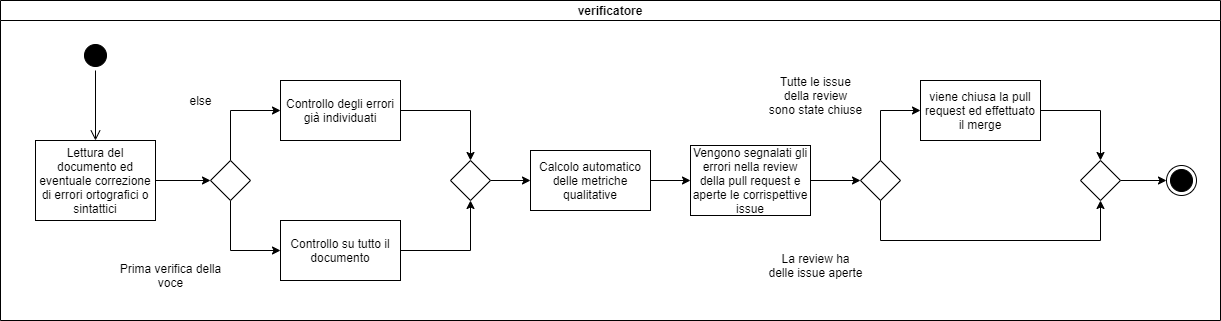
\includegraphics[width=1.0\textwidth]{../_template/images/verifica.png}
	        \caption{diagramma di attività della verifica della documentazione}
	    \end{figure}
	
	\subsubsection{Verifica del codice}
	\myparagraph{Analisi statica}
	L'analisi statica viene facilitata dall'utilizzo di ESlint, impostato secondo le norme di stile Airbnb.
	\myparagraph{Analisi dinamica}
	L'analisi dinamica viene svolta tramite l'ausilio di test, con lo scopo di verificare che il prodotto rispetti le specifiche di progettazione.
	Per tutti i test si definicono:
	\begin{itemize}
	    \item \textbf{Ambiente d'esecuzione}: ambiente hardware e software dove viene eseguito il test;
	    \item \textbf{Stati iniziali}: le configurazioni iniziali con i quali il viene eseguito;
	    \item \textbf{Input};
	    \item \textbf{Output}: output aspettato corrispondente ad un determinato input;
	    \item \textbf{Istruzioni aggiuntive}: altre istruzioni riguardanti l'interpretazione dei risultati del test e la sua esecuzione.
	\end{itemize}
	I test vengono eseguiti tramite il framework jest.js
	\myparagraph{Approcci}
	ci sono due tipi di approcci ai test:
	\begin{itemize}
	    \item \textbf{Black box}: il test ha come scopo l'appurare il comportamento del programma. Ad un determinato vettore di input, se il vettore di output è quello desiderato, il test viene considerato passato. La struttura del codice non è conosciuta dall'esecutore del test; 
	    \item \textbf{White box}: il test viene pianificato tenendo conto della struttura del codice, con l'obbiettivo, oltre a verificare il corretto funzionamento, di testare e migliorare l'efficienza e la struttura stessa. 
	\end{itemize}
	\myparagraph{Tipi di test}
	Ci sono vari tipi di test, di seguito un elenco delle tipologie d'interesse:
	\begin{itemize}
	    \item \textbf{Test di unità}: I test di unità sono di tipo White box; vengono eseguiti su unità si software individualmente per testare il corretto funzionamento e per verificare che soddisfino i requisiti di design;
	    \item \textbf{Test di integrazione}: I test d'integrazione mirano a testare il corretto funzionamento di gruppi di unità, a loro volta già testate, verificando che rispettino i contratti d'interfaccia. Un insieme di unità che supera i test d'integrazione viene considerato come una nuova unità;
	    \item \textbf{Test di sistema}: il software viene compilato come prodotto ed è testato nella sua interezza. Vengono testate le funzionalità, la performance e ci assicura che vengano soddisfatti tutti i requisiti;
	    \item \textbf{Test di accettazione}: il prodotto viene testato assieme ad i proponenti per verificare il gradimento dell'utente. Se viene superato il prodotto viene rilasciato.
	    \item \textbf{Test di regressione}: Ogni volta che viene apportata una modifica ad un'unità del software vengono rieseguiti tutti i test già definiti per verificarne il corretto funzionamento.
	\end{itemize}
	Ad ogni test di accettazione e di sistema corrisponde il seguente codice identificativo:\\
	
	\centerline{\textbf{T[tipoTest][classeRequisito][tipoRequisito][identificativo].[specializzazione]}}
	
	che è composto da:
	\begin{itemize}
	    \item \textbf{tipoTest}: può essere:
	    \begin{itemize}
	        \item \textbf{S}: test di sistema;
	        \item \textbf{A}: test di accettazione;
	    \end{itemize}
	    \item \textbf{classeRequisito}: indica la classe del requisito corrispondente, può essere:
	        \begin{itemize}
	            \item \textbf{O}: obbligatorio;
	            \item \textbf{F}: facoltativo;
	            \item \textbf{D}: desiderabile;
	        \end{itemize}
	   \item \textbf{tipoRequisito}: indica il tipo del requisito corrispondente, può essere:
	        \begin{itemize}
	            \item \textbf{F}: requisito funzionale;
	            \item \textbf{V}: vincolo;
	            \item \textbf{Q}: requisito di qualità;
	            \item \textbf{P}: requisito prestazionale. 
	        \end{itemize}
	  \item \textbf{identificativo}: identificativo progressivo del requisito;
	  \item \textbf{specializzazione}: identificativo progressivo della specializzazione.
	\end{itemize}
	Ad ogni test di unità , integrazione e regressione corrisponde il seguente codice identificativo:\\
	
	\centerline{\textbf{T[tipoTest][identificativo]}}
	
	che è composto da:
	\begin{itemize}
	    \item \textbf{tipoTest}: può essere:
	    \begin{itemize}
	        \item \textbf{U}: test di unità;
	        \item \textbf{I}: test di integrazione;
	        \item \textbf{R}: test di regressione.
	    \end{itemize}
	  \item \textbf{identificativo}: identificativo univoco progressivo.
	\end{itemize}
	\subsubsection{Metriche}
	Di seguito vengono elencate le metriche inerenti alla qualità del processo di \textbf{Verifica}. I valori sono normati nel piano di qualifica. La modalità di rilevazione non è indicata per tutte le metriche: tale dato sarà inserito in fasi successive del progetto.
	    \myparagraph{Code coverage}
        Indica il valore percentuale in centesimi del numero di righe di codice testate.
        \subparagraph{Formula}
        \begin{displaymath}
          CC = \frac{\textrm{Testate}}{\textrm{Totali}}
        \end{displaymath}
        Dove:
        \begin{itemize}
        \item[] $CC =$ Code coverage
        \item[] $\textrm{Testate} =$ numero di righe testate
        \item[] $\textrm{Totali} =$ numero di righe totali
        \end{itemize}
        
        
        \myparagraph{Numero di test superati}
        Indica il numero totale intero di test superati. Questa metrica non ha formula in quanto il valore è dato dal calcolo del programmatore in fase di test del codice.
	
	   \subsubsection{Procedimento di verifica del codice}
		Di seguito viene allegato il diagramma di attività riguardante la verifica del codice:
		\begin{figure}[hbt!]
	       \centering 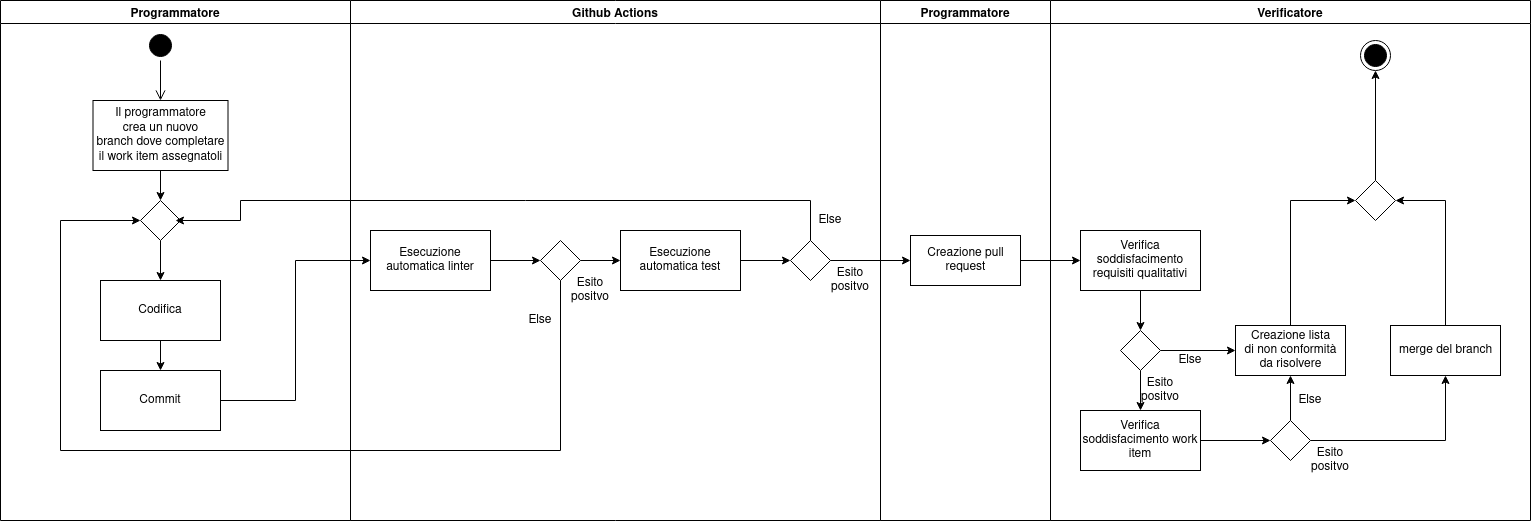
\includegraphics[width=1.0\textwidth]{../_template/images/verificaCodice.png}
	        \caption{diagramma di attività della verifica della documentazione}
	    \end{figure}

	\subsection{Validazione}

	\subsubsection{Scopo}
	La validazione è il processo che si occupa di stabilire se il prodotto soddisfi o meno i requisiti funzionali richiesti. 
	
	\subsubsection{Aspettative}
		Un prodotto validato garantisce che esso soddisfi i requisiti proposti e che soddisfi i bisogni del committente.
	
	\subsubsection{Descrizione}
	L'input per la fase di Validazione è l'output della fase di Verifica. Il compito viene poi demandato al \textit{Responsabile di progetto} il quale potrà accettare ed approvare il prodotto, oppure, rimandarlo alla fase di Verifica.
	\subsubsection{Attività}
	Per il processo di validazione vengono definite le seguenti attività:
	\begin{itemize}
	    \item \textbf{Piano di validazione}: vengono definiti gli oggetti del processo di validazione, le attività da svolgere, gli orari, gli esecutori della validazione e i documenti con i risultati;
	    \item \textbf{Test}: vengono definiti i test da condurre, assicurandosi che rispecchino i requisiti da analizzare;
	    \item \textbf{Implementazione della validazione}: il piano viene implementato ed eseguito;
	    \item \textbf{Risultati}: i risultati vengono analizzati, assicurandosi che riflettano le aspettative.
	\end{itemize}
	
	\subsubsection{Procedimento di validazione della documentazione}
		Di seguito viene allegato il diagramma di attività riguardante la validazione della documentazione:
		\begin{figure}[hbt!]
	       \centering 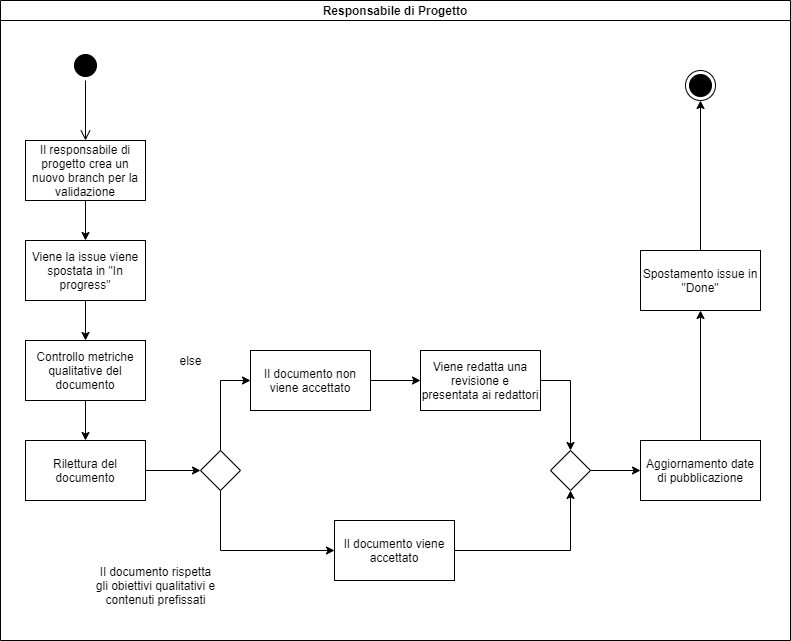
\includegraphics[width=1.0\textwidth]{../_template/images/Validazione.png}
	        \caption{diagramma di attività della validazione della documentazione}
	    \end{figure}
	   
	\subsubsection{Procedimento validazione del codice}
	    di seguito viene allegato il diagramma di attività riguardante la validazione del codice:
	    \begin{figure}[hbt!]
	       \centering 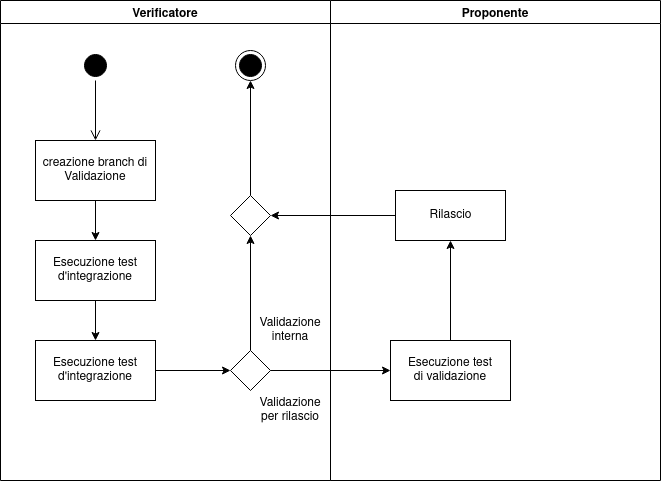
\includegraphics[width=1.0\textwidth]{../_template/images/validazioneCodice.png}
	        \caption{diagramma di attività della validazione della documentazione}
	    \end{figure}
